\pdfminorversion=4
\documentclass[]{article}
\usepackage[utf8]{inputenc}
\usepackage{amssymb,latexsym,amsmath}
\usepackage[a4paper,top=3cm,bottom=2cm,left=3cm,right=3cm,marginparwidth=1.75cm]{geometry}
\usepackage{graphicx}
\usepackage[colorlinks=true, allcolors=blue]{hyperref}
\usepackage{float}

\title{ECE271 Final Design}
\author{Drew Ortega, Jonathan Alexander, Cole Swanson}
\date{\today}

\begin{document}
\begin{titlepage}
    \begin{center}
        \vspace*{1cm}
 
        \Huge
        \textbf{ECE272 Final Design}
 
        \vspace{0.5cm}
        \LARGE
        Controller Input and VGA
 
        \vspace{1.5cm}
 
        \textbf{Drew Ortega}
        
        \textbf{Cole Swanson}
        
        \textbf{Jonathan Alexander}
 
 		\vspace{0.5cm}
        \today
 
    \end{center}
\end{titlepage}

\newpage
	\tableofcontents
\newpage

\section{Introduction}
Some introduction Text Here

\section{Design}
Some design text here
\subsection{Item1Title}
Some Subsection here
\subsection{SecondSub Section}
Other Subsecion Here
\section{Controllers}
\subsection{NES/SNES Controller}
The NES and SNES controllers utilize three lines to transfer data, along with a ground and 5V power supply. Communication wit the controllers uses a data latch line, clock line and data line. The clock and data latch lines are supplied to the controller, while the data line is generated. When the latch line is driven high, the controllers log the pressed buttons within an active low shift register. The first bit of this register is automatically output on the data line. Whenever the clock input is cycled, the shift register moves along by one bit. The NES controller has eight buttons, and an eight bit shift register, while the SNES has sixteen buttons and a sixteen bit shift register. The data latch can then be cycled to obtain a new set of inputs. For this design, the up, down, left, and right inputs were of interest. Within the NES controller, the zeroth bit of the shift register corresponds to the right input, the first to  the left input, the second to the down input, and the fourth to the up input. The final four inputs were ignored. Within the SNES controller, the up input corresponds to the fifth bit in the shift register, the down input to the sixth bit, the left input to the seventh bit, and the right input to the eight bit. \\~\\
To communicate with the NES or SNES controllers, the host must do the following:
\newline
1. Drive the data latch input high to populate the shift register
\newline
2. The first data bit can now be read
\newline
3. The clock input should be driven high, then low
\newline
4. The next data bit can now be read
\newline
5. Steps 3-4 should be repeated 7 times for the NES, 15 times for the SNES(as the first bit of the register is already present, one less clock cycle is needed)

\section{HDL Modules}
\subsection{NES/SNES input decoder}
\begin{figure}[H]
	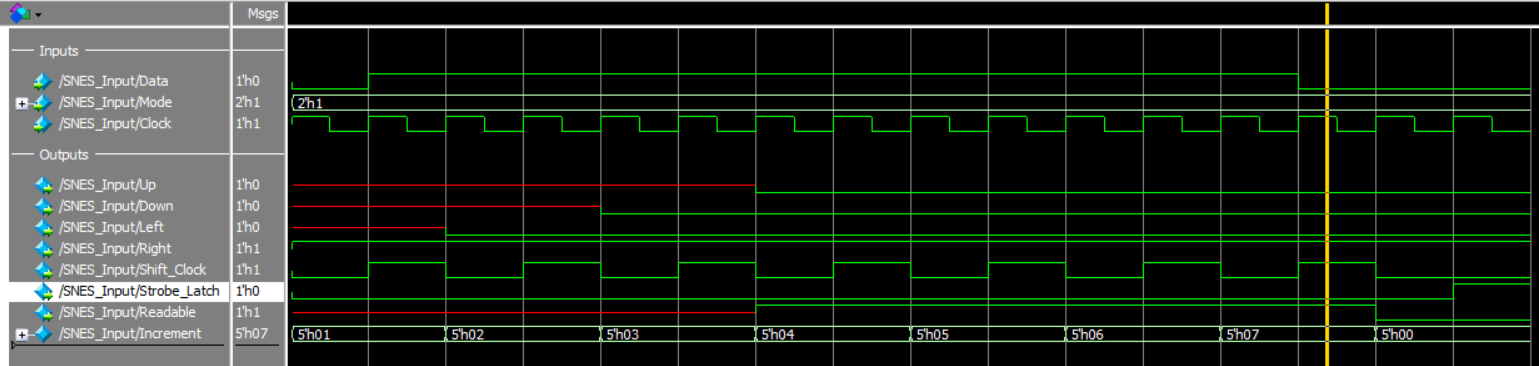
\includegraphics[width=\linewidth]{NES_Input_Sim.png}
	\caption{ModelSim of the NES/SNES controller decoder in NES mode.}
\end{figure}

\begin{figure}[H]
	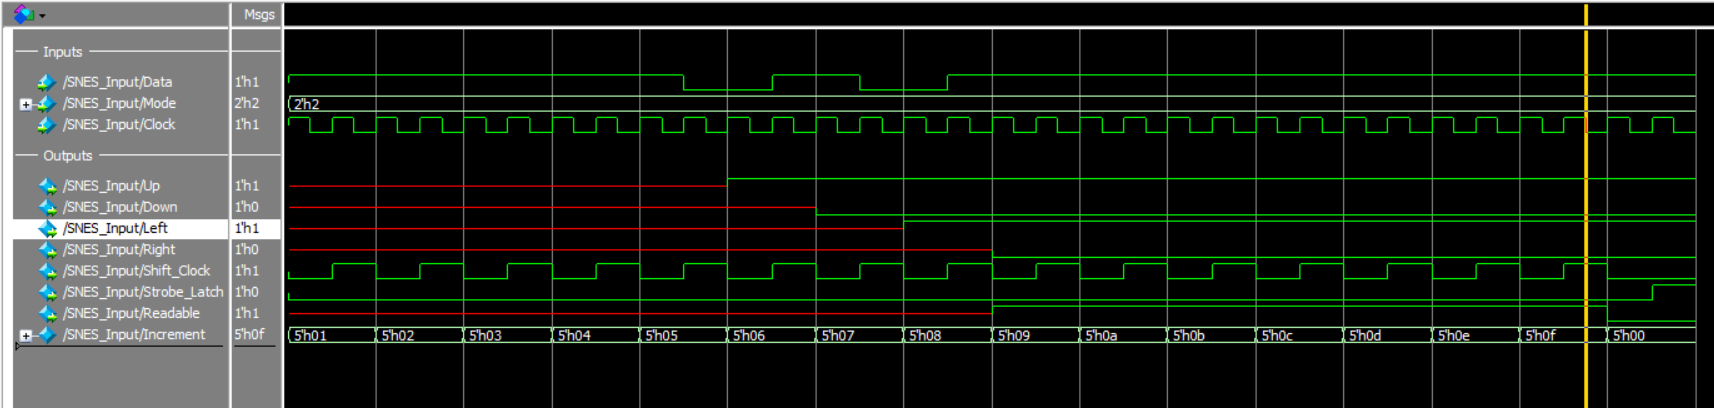
\includegraphics[width=\linewidth]{SNES_Input_ModelSim.png}
	\caption{ModelSim of the NES/SNES controller decoder in SNES mode}
\end{figure}
Inputs: One bit data representing the current bit from the controller shift register, one bit clock, and two bit mode used to determine which controller is in use(NES or SNES)\\~\\
Outputs: One bit up, down, left, and right representing the decoded values from the controller, and one bit readable output which is driven high once the current set of values have been decoded. Also present are the one bit strobe latch output, which functions as the data latch for the controller to be driven high then low to log the inputs to the controller, and a one bit shift clock, which is used to shift the values in the controller shift register. \\~\\
Simulations: \\~\\
NES: \\
For this simulation, the data bit for right was driven low(representing an input of 'right'). The data\_latch is initially driven high. As expected, the decoder logs the right input as pressed, and continues through the inputs by providing a shift\_clock to the controller. Once the data has been cycled three times, all values of interest are accounted for, and the readable output is driven high. After seven cycles of the output, the data\_latch is again driven high and readable is driven low; new inputs are ready to be read. The value of increment represents the current bit of the shift register.\\~\\
SNES: \\
For this simulation, the data bits for up and left were driven low(representing inputs of 'left' and 'up'). The data\_latch is initially driven high. As expected, the decoder logs the up and left inputs as pressed, and continues through the inputs by providing a shift\_clock to the controller. Once the data has been cycled eight times, all values of interest are accounted for, and the readable output is driven high. After fifteen cycles of the output, the data\_latch is again driven high and readable is driven low; new inputs are ready to be read. The value of increment represents the current bit of the shift register.\\~\\
This module will use the system clock to drive its logic. On the first clock cycle, the data latch output will be driven high to log the controller inputs. The data latch will then be driven low, and the shift clock will be cycled seven times for the NES controller, or fifteen times for the SNES controller, with the bit corresponding to the inputs of interest recorded. Once all inputs of interest have been recorded, the readable output will be driven high, signaling all inputs are accounted for. Pressed buttons on the controllers will be signaled by a high value on the corresponding output from the decoder(up, down, left, or right). 
\subsection{Game Logic Controller}
\begin{figure}[H]
	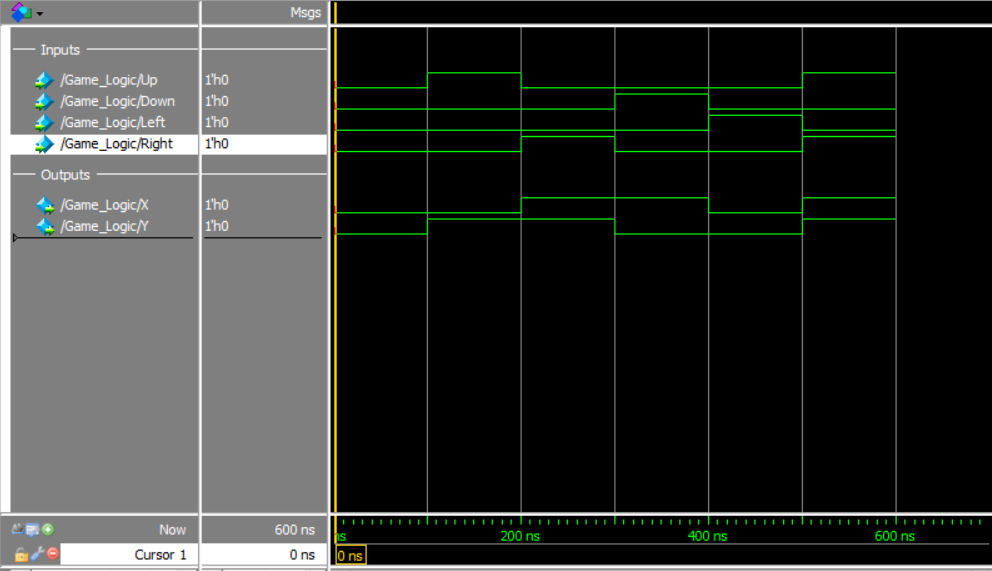
\includegraphics[width=\linewidth]{Game_Logic_ModelSim.png}
	\caption{ModelSim of the Game Logic Controller.}
\end{figure}
Inputs: One bit inputs for up, down, left, and right\\~\\
Outputs: One bit data inputs for X and Y, representing the position of the player object within the four by four grid where 0,0 is the lower left corner \\~\\
Simulation: \\~\\
Within this simulation, the initial position of the player, 0,0. The up input is driven high, and as expected the coordinate output for Y also changes to high. Next, a right input is provided, and again the coordinates change such that X is high. After this, down is driven high and then left is driven high, resulting in the coordinates shifting to 0,1 then 0,0. Finally, both up and right are driven high, resulting in a coordinate of 1,1.\\~\\
This module will use combinational logic to determine the coordinate state of a player. The current position is stored within the module, and from the provided values of up, down, left, and right the next position is determined. An input that would result in the player going outside of the coordinate bounds(0,0 to 1,1) is ignored. Multiple inputs can be accepted at once, allowing for diagonal movement.  


\end{document}